\section{Constructing topics using human judgments}
\label{sec:tasks}
In this section we propose a task which creates a formal setting where
humans can create a latent space representation of the corpus.  Our
task, \emph{tag-and-cluster}, replaces the collapsed Gibbs sampling
step of \myeq{eq:sampling} with a human judgment.  In essence, we are
constructing a gold-standard series of samples from the
posterior.\footnote{Additionally, since Gibbs sampling is by nature
  stochastic, we believe that the task is robust against small
  perturbations in the quality of the assignments, so long as in
  aggregate they tend toward the mode.}

\begin{figure*}
\centering
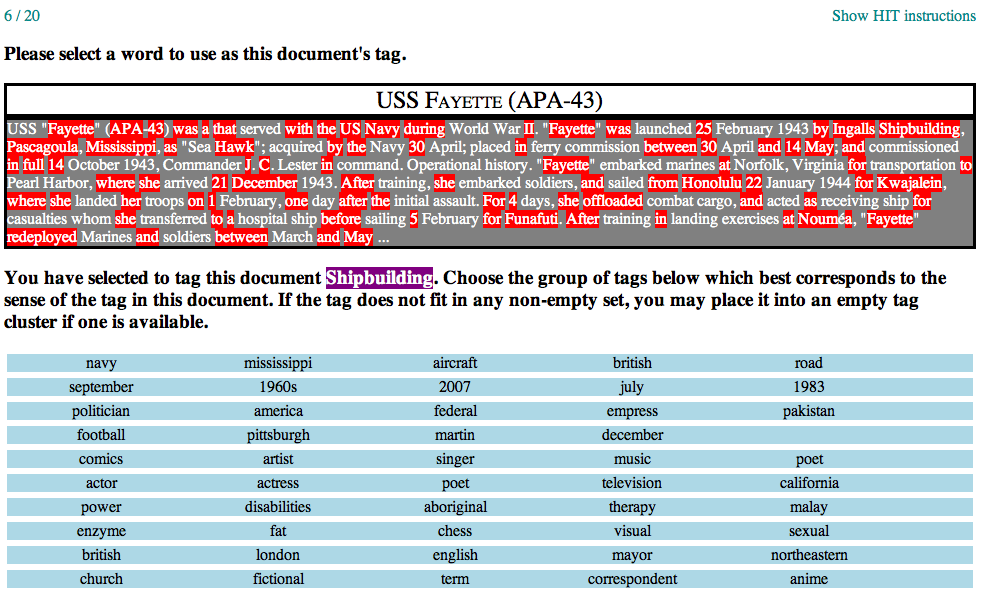
\includegraphics[width=0.80\textwidth]{figures/screenshots.png}
\caption{Screenshots of our task.  In the center, the document along
  with its title is shown.  Words which cannot be selected, e.g.,
  distractors and words previously selected, are shown in red.  Once a
  word is selected, the user is asked to find a topic in which to
  place the word.  The user selects a topic by clicking on an entry in
  a menu of topics, where each topic is expressed by the five words
  which occur most frequently in that topic.}
\label{fig:screenshot}
\end{figure*}

Figure~\ref{fig:screenshot} shows how \emph{tag-and-cluster} is
presented to users.  The user is shown a document along with
its title; the document is randomly selected from a pool of available
documents.  The user is asked to select a word from the document which
is discriminative, i.e, a word which would help someone looking for
the document find it.  Once the word is selected, the user is then
asked to assign the word to the topic which best suits the sense of
the word used in the document.  Users are specifically instructed to
focus on the meanings of words, not their syntactic usage or
orthography.

The user assigns a word to a topic by selecting an entry out of a menu
of topics.  Each topic is represented by the five words occuring most
frequently in that topic.  The order of the topics presented to the
user is determined by the number of words in that document already
assigned to each topic.  Once an instance of a word in a document has
been assigned, it cannot be reassigned and will be marked in red when
subsequent users encounter this document.  In practice, we also
prohibit users from selecting infrequently occurring words and stop
words.


